\chapter{Research Methodology}
This chapter provides a detailed exposition of the methodology used throughout this work. This study has conducted exploratory and descriptive research to determine whether the use of simulation and an automated feedback driven system, a user can be trained as a race driver. The chapter is structured as follows: \S~\ref{sec:meth-overview} provides a general overview of the overarching methodology used in the study, \S~\ref{sec:meth-experiment-setup} describes in length the design of the instrument used to acquire experiment data and results, \S~\ref{sec:meth-experiment-structure} presents the experimental procedure and the rationale behind it, \S~\ref{sec:meth-data-gathering} identifies the information and data acquired through the experimental and descriptive methodologies employed, and finally \S~\ref{sec:meth-data-analysis} presents the data analysis mechanisms employed to substantiate our conclusions.
%
% Overview
%
\section{Overview}
\label{sec:meth-overview}
This study conducted experimental and descriptive research on the viability of the use of simulators in conjunction with an automated feedback system for improving race driving skills in the normal population. Specifically, a user study was devised and carried out with the primary goals being:
\begin{enumerate}
	\item To determine whether a context-based feedback system can improve the skills of a participant
	\item To quantify the magnitude of this improvement, if (1) is true
\end{enumerate}

These goals were addressed by means of an experimental setup based on a race-driving simulator, using which objective measurement of the participant performance could be gathered and analysed, and a questionnaire for relating the participant's experience with the experimentally-gathered data. The setup of the experiment is explored in more detail in \S~\ref{sec:meth-experiment-setup}.

Since the main goal of this study is that of assessing how effective a feedback system is in the learning process, the independent variable in the experiment is the ability to receive feedback. The hypothesis is that participant performance (such as average lap time) is improved through feedback, and is thus a dependent variable. However, practising without feedback can also lead to changes in the dependent variable; therefore this is controlled for by having two groups of participants: the experimental group that receives feedback and the control group that doesn't. Random assignment is used to determine a participant's group.

A questionnaire, to be administered to the participants at the end of the session, will be designed to help normalise and control for other factors that may influence dependent variables, and hence, the outcome of the experiment. The design of the questionnaire also helps in bridging the participants' perception of their performance with the actual performance data, possibly providing further insight into the results. A questionnaire was preferred to an interview because it is easier to administer, it lends itself to group administration and also allows confidentiality. It is indeed true that interviews permit a greater freedom of expression on behalf of the participant; however, questionnaires create a sense of anonymity that encourages the participants to be more truthful in their answers \cite{introductiontobehavioralresearchmethods}.

\section{Experiment Design}
\label{sec:meth-experiment-design}
In the experiment, each group would be utilising the same car and racetrack. Bastow et al. \cite{bastow2004car} suggest that cars equipped with a front wheel drivetrain may be easier to handle. The Fiat 500 Abarth was the car chosen for the experiments, partially based on Bastow et al.'s findings. The car is relatively low-powered and thus, easier to use by beginning drivers. The Silverstone National race track has the desirable properties of being flat and smooth, without uneven surfaces or bumps which may result in loss of control in rookie drivers. Furthermore, the way the track is structured, with wide run-off areas located along the circuit where drivers are most likely to lose control of the car, allows the car to slow down before colliding with barriers or other stationary objects.

Two feedback mechanisms have been considered for this experiment, \emph{visual}, through the use of a heads-up-display (HUD) superimposed on the simulation display, or \emph{auditory}, by means of descriptive speech projected through loud speakers. Leahy et al. \cite{leahy2003auditory} argue that auditory feedback is less intrusive that visual clues; based on these findings, it was decided that the system should provide feedback using auditory clues.

\begin{figure}
	\centering
	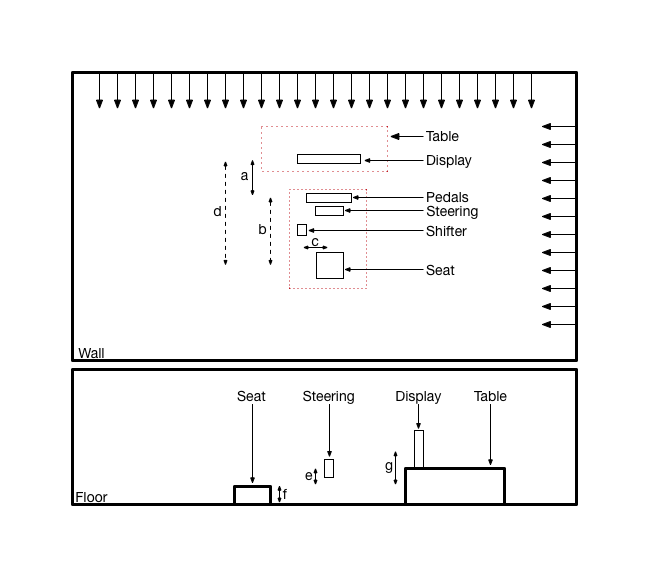
\includegraphics[width=\textwidth]{images/experiment-setup-schematic.png}
	\caption[Experiment Setup Schematic]{Top-down and side views of experiment setup}
	\label{fig:meth-experiment-setup}
\end{figure}

\section{Experiment Materials}
\label{sec:meth-experiment-setup}
The setup of the experiment was divided into three material categories: \emph{simulation environment}, \emph{simulation hardware} and \emph{simulation software}, with each category subscribing to a number of desirable properties: 

\begin{description}
	\item [Environment] The experiment should be carried out in an isolated, noise-free and well-lit room. Participants would be let in the room one at a time, to ensure the experiment is conducted without any distractions.
	\item [Hardware] The hardware components identified for this experiment are the (i) display output, (ii) audio output, (iii) steering wheel, (iv) gear shifter, (v) acceleration, brake and clutch pedals and (vi) seating frame.
	\begin{description}
		\item [Display and Audio] 32 inch lcd display capable of 1080p resolution with integrated stereo audio output.
		\item [Driving Controls] The driving controls include (ii)-(iv); minimally a steering wheel should provide the same number of revolutions as a racing car, providing accurate force feedback to let the participants accurately assess the behaviour of the car. Gear shifters do not implement feedback mechanisms; however, given their ubiquity, H-shifters are preferred since they are the kind most drivers are familiar with. High-end pedal systems use hydraulics to simulate the variability of force required on part of the driver to actuate a pedal during different stages.
		\item [Seating frame] The seating frame should ensure a seating position akin to a driver in a racing car. The seating frame should also provide the ability to move the seat back and forward inorder for participants to be able to seat comfortable and be able to reach the pedals.
	\end{description}
	\item [Software] The chosen sim racing game must include (i) realistic driving model, (ii) real life tarmac circuits (iii) ability to disable wear and tear on the car, (iv) quality of graphics and most importantly (v) provide means to read telemetry data while also being easy to interface to.
	\begin{description}
		\item [Real life tarmac circuits] Most sim games replicate accurately tracks, including elevation changes, bumps and distances. By having the level of realism, participants can be exposed to real life scenarios. The circuits also need to be a loop so that participants do not need to reset the game to do another lap,  which could be tedious. 
		\item [Ability to disable wear and tear] This is important as it allows for better controlling of experiment variables as cars will not get progressively worse during a session hindering a participants.
		\item [Quality of graphics] The game should be visually appealing in order to provide the right level of impressions. Sim games might prefer to allocate more processing power to the physics engine which ipects the quality of the graphics produced. In the case of the project good graphics will be given a slight preference.
		\item [Read telemetry data] In order for feedback to be given out, it must be possible to be able to know what the car is doing on track. This is achieved by having the sim game allow 3rd party software to read the telemetry data.
	\end{description}
\end{description}

\subsection{Hardware choice}

The comparison table shows the desired properties the steering wheel controls should have. The G25 is the only which comes as a bundle with a three pedal set and H shifter on top of that, it's also the cheapest. The Toastmaster TX and Fanatec are more high end which explains the spike in price. These two to not come with a three pedal set nor an H shifter but can be purchased separately for an extra cost. The G25 is the obvious choice given it's relative low cost and the ability to supply decent force feedback.

\begin{center}
	\begin{tabular}{ | l | l | l | l |}
		\hline
						& G25			& Trustmaster TX	& Fanatec 		\\ \hline
		Cost ( EUR )	& 240 			& 324 				& 499 			\\ \hline
		900' turn		& \checkmark 	& \checkmark 		& \checkmark	\\ \hline
		Three pedal set	& \checkmark 	&  					& 				\\ \hline
		H Shifter 		& \checkmark 	&			 		&				\\ \hline
		Force Feedback	& \checkmark 	& \checkmark 		& \checkmark	\\ \hline
	\end{tabular}
\end{center}

\subsection{Software choice}

The comparison table shows the desired properties a sim game must have, and a selection of games which have been considered. Fromt he start it is clear, Dirt and Forza Motorsport 6 should be discarded as none provided telemetry data to be read. Assetto Corsa, Project Cars and iRacing are closely matched, however Assetto Corsa has the leading edge as it provides an easy way to interface via UDP, well document and wide developer community who can help. Furthermore Assetto Corsa provides good visual graphics. For these reasons Assetto Corsa has been picked as the game to be used.

\begin{center}
	\begin{tabular}{ | l | l | l | l | l | l |}
		\hline
			& Assetto Corsa & Project Cars & iRacing & Dirt & Forza Motorsport 6 \\ \hline
		Realistic model	& \checkmark &\checkmark & \checkmark & \checkmark & \checkmark \\ \hline
		Tracks	& \checkmark &\checkmark & \checkmark &  & \checkmark \\ \hline
		Disable wear & \checkmark & \checkmark & \checkmark & \checkmark & \checkmark \\ \hline
		Telemetry data	& \checkmark & \checkmark & \checkmark &  &  \\ \hline
		Ease of Interfacing	& \checkmark &  & \checkmark &  &  \\ \hline
		Quality of graphics & \checkmark & \checkmark &  & \checkmark & \checkmark \\ \hline
	\end{tabular}
\end{center}

\subsection{Questionnaire}
Questionnaires allow for further insight from the point of view of the participants. Leary et al. provide seven guidelines for compiling a questionnaire \cite{introductiontobehavioralresearchmethods}:
\begin{enumerate}
	\item being specific and precise in phrasing the questions
	\item writing the questions as simply as possible, avoiding difficult words, unnecessary jargon, and cumbersome phrases
	\item avoid making unwarranted assumptions about the respondents
	\item conditional information should precede the key idea of the question
	\item do not use double-barrelled questions
	\item pretest the questions
\end{enumerate}
Responses from questionnaires designed using these guidelines are valid in the general case. The challenge in choosing a response format in a question lies in identifying whether one should go for an open ended question in which more information might be collected, or on the other hand, use a rating scale response format, where the response is more constrained but may be easier to analyse. Leary et al. suggest using the former for questions dealing with behaviours, thoughts, or feelings that can vary in frequency or intensity (e.g. the Likert Scale\cite{likert1932technique}) and using open ended questions in cases where further insight is desired.

Based on these guidelines two qualitative questionnaires have been designed, one aiming to gather insight into the sample demographic, the other aiming to gain insight into the participants' impressions about the realism of the experiment setup, the level of comfort, or discomfort and any suggestions or comments they might have. 

\subsection{Participants' Demographic}

\subsection{Participants' Insight}

\section{Procedure}
\label{sec:meth-experiment-structure}
In order to evaluate the effectiveness of the system a user study took place. Participants were split randomly into two groups. One group will be referred as the feedback group, the other will be referred to as the base group. The experiments structure was subdivided into smaller systemic tasks.

\begin{description}
	\item[Demographic questionare] At the start on the experiment the demographic questionare is to be handed out to the participant.
	
	\item[Adjust Rig Configuration] In order for the participant to sit comfortable while also ensuring all controls can be reached with ease, the rig has to be configured per participant. This involves having to move the seat further back or forward to the steering wheel, as it would be done in a real car. In addition participants are also told how to operating the rig. The explanation covers the steering wheel turns two and a half turns from lock to lock, the pedals are setup as on any manual road car, having the clutch pedal on the left, brake in the middle, and throttle on the right. The H shifter is also explained by having a run through demonstration of all gears which allows participants to be able to operate the rig with out having to learn on their own.
	
	\item[Breaks] To avoid having driving sessions possibly put too much strain on participants, optional five minute breaks are allowed to be taken between driving sessions. 
	
	\item[Ten minuties practice] During these ten minutes users are told to simply get used to the rig setup, track and car. The aim of this session is for participants to get used to the setup while also allow this study to measure their skill before the feedbvack system as the independent variable is introduced.
	
	\item[Two Ten minuties sessions] These are the sessions in which the feedback system is turned on for the feedback group, while the participants in base group are left to keep trying to improve without any aid. 
	
	\item[Five minuties session] A final five minuties of driving are allocated yet again, this time with the feedback system turned of for both groups. This was designed to possibly identify any conclusive results. Such session could show the possibility of the feedback group performing worst after having the aid of the feedback system removed or both groups ending up performing the same after the sessions, which would suggest the feedback participant didn't manage to get any cognitive advantage.
	
	\item[Particpant's feedback questionare] The final stage of the experiment requires participants to fill in the a questionnaire  in which they are asked to give their feedback on the experiment structure, hardware used and any further comments they would like to add.
	
\end{description}

\section{Data Collection and Sampling}
\label{sec:meth-data-gathering}
At the end of the experiments the data collected includes two questioners from each participant and four batches of telemetry data, one for each participant. Questioners are filled online using Google Forms as it provides the ability to export the data and also automatic generation of descriptive statistic. The data collected from the questionnaires and telemetry data is to be loaded into a data base management system from which the data can be queried using specialised data querying constructs. By having a querying language, it provides the flexibility of extract data which is relevant for the data analysis at hand.

\section{Data Analysis}
\label{sec:meth-data-analysis}
In order to accept or reject the null hypothesis statistical test are to be carried out. Most important is the ability to compare the performance of the two groups across sessions. The lap time is used as the test variable as this gives a good indication for the average performance achieved during a lap. Furthermore which comparison test to use depends on the the sample size, the distribution of data and the types of group. In this case the groups are independent from each other, as a participant may not be part of the base group and also part of the feedback group. As pointed out by De Smith in his book "Statistical Analysis Handbook-a web-based statistics" the tests of interest to this project are the Independent samples t-test\cite{de2015statsref} and the Mann Whitney U test\cite{de2015statsref} as the these test for difference between independent groups. Both tests share the same hypothesis listed below.

\begin{description}
	\item[Independent t test] assumes the data is normally as such the data must be check for normal distribution. This can be carried out by using the Shapiro-Wilk\cite{de2015statsref} test for normality on both groups.
	
	\item[Mann Whitney U test] Does not require the data to be normally distributed but it assumes the groups' data shares the same distribution. The groups are checked for equal distribution using the Independent Samples Kolmogorow-Smimov test.
	
	\item[Null hypotesis]there is no significant difference across the groups
	\item[Alternative hypotesis]there is significant difference across the groups
\end{description}

As the data distribution is not known before hand, distribution test will be carried out after the data is collected and depending on the result, the adequate test will be used.